% Extraído de Textuais/03-Metodologia.tex
% Fonte: 5-Coleta_features/conferencia_git_log_L/exemplo_mylyn_createAdditionalControls.md (2026-11-09).
\begin{figure}[htbp]
    \captionsetup{font+={color=ForestGreen}}%
    \caption{Commits do método \texttt{create\-Additional\-Controls} do Mylyn contados pela coleta e listados pelo \texttt{git log -L}}
    \label{fig:met-gitlog-intersecao}
    \centering
    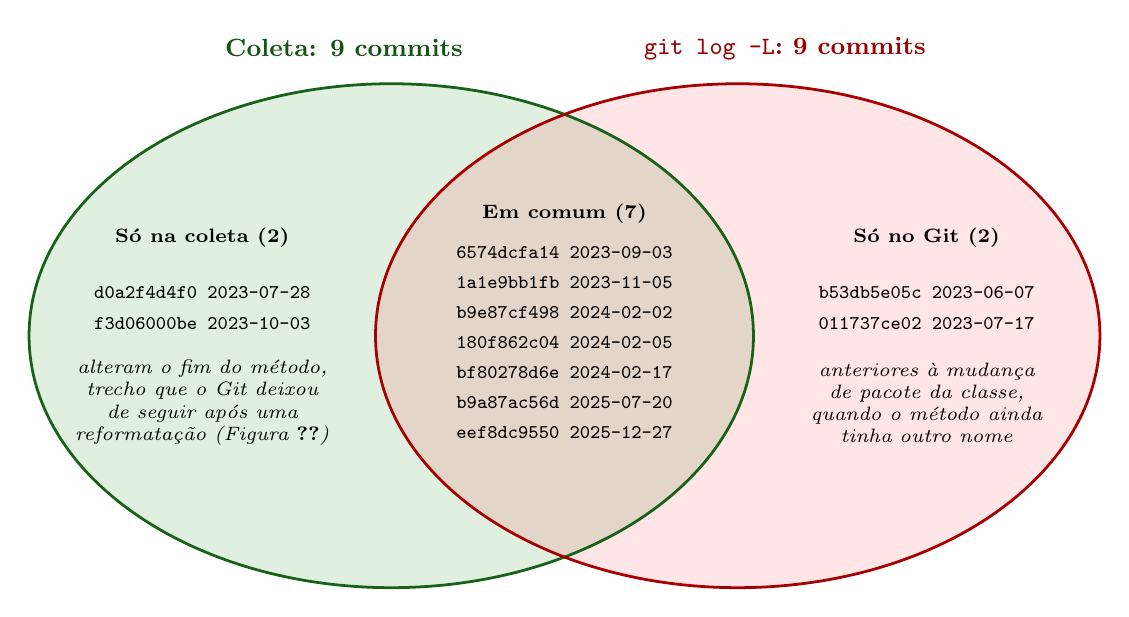
\begin{tikzpicture}[font=\scriptsize,
        cid/.style={font=\scriptsize\ttfamily,inner sep=0pt},
        tit/.style={font=\small\bfseries,align=center},
        reg/.style={font=\scriptsize\bfseries,align=center},
        nota/.style={font=\scriptsize\itshape,align=center,text width=3.4cm}]
        % conjuntos
        \fill[ForestGreen,fill opacity=0.14] (0,0) ellipse [x radius=4.6cm, y radius=3.2cm];
        \fill[red,fill opacity=0.10] (4.4,0) ellipse [x radius=4.6cm, y radius=3.2cm];
        \draw[ForestGreen!70!black,line width=1pt] (0,0) ellipse [x radius=4.6cm, y radius=3.2cm];
        \draw[red!65!black,line width=1pt] (4.4,0) ellipse [x radius=4.6cm, y radius=3.2cm];
        % títulos
        \node[tit,text=ForestGreen!60!black] at (-0.6,3.65) {Coleta: 9 commits};
        \node[tit,text=red!60!black] at (5.0,3.65) {\texttt{git log -L}: 9 commits};
        % só na coleta
        \node[reg] at (-2.4,1.25) {Só na coleta (2)};
        \node[cid] at (-2.4,0.55) {d0a2f4d4f0 2023-07-28};
        \node[cid] at (-2.4,0.15) {f3d06000be 2023-10-03};
        \node[nota] at (-2.4,-0.85) {{\laranja alteram o fim do método, trecho que o Git deixou de seguir após uma reformatação (Figura~\ref{fig:met-gitlog})}};
        % nas duas
        \node[reg] at (2.2,1.55) {Em comum (7)};
        \foreach \c/\d [count=\i] in {6574dcfa14/2023-09-03, 1a1e9bb1fb/2023-11-05, b9e87cf498/2024-02-02,
                                     180f862c04/2024-02-05, bf80278d6e/2024-02-17, b9a87ac56d/2025-07-20,
                                     eef8dc9550/2025-12-27}
            \node[cid] at (2.2,1.05-0.38*\i+0.38) {\c\ \d};
        % só no Git
        \node[reg] at (6.8,1.25) {Só no Git (2)};
        \node[cid] at (6.8,0.55) {b53db5e05c 2023-06-07};
        \node[cid] at (6.8,0.15) {011737ce02 2023-07-17};
        \node[nota] at (6.8,-0.85) {anteriores à mudança de pacote da classe, quando o método ainda tinha outro nome};
    \end{tikzpicture}
    \fonte{Elaborado pelo autor (2026).}
\end{figure}%
